\documentclass[twoside,12pt]{book}
\usepackage{fontspec} 
\usepackage[utf8]{inputenc} 
\newfontfamily{\arial}{Arial Unicode MS}
\newfontfamily\EmojiFont{Segoe UI Emoji}[Renderer=Harfbuzz]
\newcommand{\emoji}[1]{{\EmojiFont #1}}
% 默认字体保持LaTeX标准设置
% 中文支持设置
% 使用ctex包但不使用默认字体设置(fontset=none)
\usepackage[fontset=none]{ctex}
% 设置中文字体:宋体为主字体,黑体为粗体,楷体为斜体
\setCJKmainfont{SimSun}[
  BoldFont = SimHei,
  ItalicFont = KaiTi,
  BoldItalicFont = KaiTi
]

% 加载常用包
\usepackage{tcolorbox}  % 彩色文本框支持
\usepackage{ulem}
\tcbuselibrary{skins, breakable}  % 加载tcolorbox的皮肤和断页功能
\usepackage{tikz}  % 绘图支持
\usepackage{graphicx}  % 图片插入支持
\graphicspath{{figures/},{figures/部门1/},{figures/部门2/},{figures/看板/},{figures/头像/},{figures/部酱/},{figures/页眉页脚/}}  % 设置图片路径为figures目录
% 颜色和页面布局设置
\usepackage{xcolor}  % 颜色支持
\usepackage{wrapfig}  % 文字环绕图片支持
\usepackage{floatflt}
\usepackage{eso-pic}  % 页面背景支持
\usepackage{geometry}  % 页面布局设置
\usepackage{setspace}
\usepackage{textcomp}
%\usepackage{showframe}
\usepackage{pifont}
\usepackage{fancyhdr}
\usepackage{comment}
\usepackage{adjustbox}
\usepackage{eso-pic}
\usepackage{ragged2e}
\usepackage{tikz}
\usetikzlibrary{shapes.geometric}
\usepackage{multicol}
\usepackage{enumitem}
\newenvironment{categorysection}[1]{
  \subsection*{\textcolor{truepurple}{#1}}
  \begin{itemize}[leftmargin=*, 
                 nosep,               % 移除所有额外间距
                 itemsep=2pt,         % 条目间距=0
                 parsep=0pt,          % 段落间距=0
                 before=\setlength{\baselineskip}{23pt} % 设置行距
  ]
}{
  \end{itemize}
}
\usetikzlibrary{calc,positioning}
\usetikzlibrary{shapes, arrows}  

\geometry{a4paper, left=1.5cm, right=1.5cm, top=2cm, bottom=2.5cm}
% 设置无衬线中文字体为黑体
\setCJKsansfont{SimHei}

% 定义文档使用的颜色
\definecolor{truepurple}{RGB}{128, 0, 128}  % 主色调紫色
\definecolor{taopink}{HTML}{F17F98}  % 桃子名字
\definecolor{tao}{HTML}{FFF2F9}  % 桃子气泡
\definecolor{zi}{HTML}{F8F2F9}  % 紫荆气泡
\definecolor{qing}{HTML}{F2F9EA}  % 清芬气泡
\definecolor{default}{HTML}{F9F9F9}  %默认气泡灰
% 加载tikz的渐变效果库
\usetikzlibrary{fadings}

% 页面布局设置
\geometry{
  top=1.5cm,       % 从3cm减小到1.5cm
  headheight=20.57637pt, % 解决fancyhdr警告
  headsep=10pt,     % 增加页眉与正文间距
  footskip=30pt     % 增加页脚与正文间距
}

% 定义聊天气泡样式
% 使用说明:
% \chatbubble[位置]{头像路径}{昵称}{消息内容}{背景颜色}
% 可选参数:
% [left] - 左侧气泡(默认)
% [right] - 右侧气泡
% 示例:
% \chatbubble[left]{taozi.png}{桃子}{消息内容}{tao}
% \chatbubble[right]{zijing.png}{紫荆}{消息内容}{zi}
% \chatbubble[right]{qingfen.png}{清芬}{消息内容}{qing}
\newcounter{chatcounter}
\newcommand{\chind}{\hspace*{2em}}
\newcommand{\chatbubble}[5][left]{%
  \stepcounter{chatcounter}%
  \par\noindent%
  \ifstrequal{#1}{left}
    {% 左侧气泡
     \begin{minipage}[t]{1.2cm} % 头像宽度
        \begin{tikzpicture}[baseline=(current bounding box.center)]
          \node[circle, draw=gray!50, line width=0.5pt, minimum size=1.2cm, 
                path picture={\node at (path picture bounding box.center) 
                {\includegraphics[width=1.2cm]{#2}};}] {};
        \end{tikzpicture}
     \end{minipage}%
     \hspace{0.2cm}%
     \begin{minipage}[t]{0.7\textwidth} % 消息框宽度
        \vspace{-15pt} % 确保顶部对齐
        \noindent\textcolor{darkgray!80}{\sffamily #3} % 昵称
        \vspace{5pt}
        \begin{tcolorbox}[
          enhanced,
          breakable=false,
          colback={#5},
          colframe={#5},
          arc=8pt,
          boxrule=0.5pt,
          left=8pt,
          right=8pt,
          top=4pt,
          bottom=4pt,
          before skip=0pt,
          after skip=10pt,
          width=\linewidth,
          before upper={\setlength{\parindent}{0em} \setlength{\parskip}{0pt}},
        ]
          #4
        \end{tcolorbox}
     \end{minipage}
    }
    {% 右侧气泡
     \hfill%
     \begin{minipage}[t]{0.7\textwidth} % 消息框宽度
        \vspace{-15pt} % 确保顶部对齐
        \noindent\hfill\textcolor{darkgray!80}{\sffamily #3} % 右对齐昵称
        \vspace{5pt}
        \hfill%
        \begin{tcolorbox}[
          enhanced,
          breakable=false,
          colback={#5},
          colframe={#5},
          arc=8pt,
          boxrule=0.5pt,
          left=8pt,
          right=8pt,
          top=4pt,
          bottom=4pt,
          before skip=0pt,
          after skip=10pt,
          width=\linewidth,
          before upper={\setlength{\parindent}{0em} \setlength{\parskip}{0pt}},
        ]
          #4
        \end{tcolorbox}
     \end{minipage}%
     \hspace{0.2cm}%
     \begin{minipage}[t]{1.2cm} % 头像宽度
        \begin{tikzpicture}[baseline=(current bounding box.center)]
          \node[circle, draw=gray!50, line width=0.5pt, minimum size=1.2cm, 
                path picture={\node at (path picture bounding box.center) 
                {\includegraphics[width=1.2cm]{#2}};}] {};
        \end{tikzpicture}
     \end{minipage}
    }%
  \par\vspace{0.1cm}% 气泡间距
}
\newcommand{\picbox}[1]{%
\vspace{0.3em}

    \begin{tikzpicture}
        \node[
            trapezium, 
            draw=truepurple, 
            fill=truepurple!80!black, 
            text=white, 
            inner sep=3pt, 
            minimum width=0.8\linewidth, % 宽度为行宽的80%
            minimum height=0.3cm, 
            trapezium left angle=90, % 左边直角
            trapezium right angle=65, % 右边角度
            trapezium stretches=true, % 允许拉伸
            align=left % 文本居左
        ] 
        {#1};
    \end{tikzpicture}%
}
% 设置页眉页脚样式
\pagestyle{fancy}  % 使用fancy页眉页脚样式
\fancyhf{} % 清空所有页眉页脚默认设置

% 设置页眉
% LE: 偶数页左侧页眉
\fancyhead[LE]{\hspace*{-1.5cm}
\includegraphics[width=\paperwidth]{head.pdf}} 
% RO: 奇数页右侧页眉
\fancyhead[RO]{\hspace*{-1.5cm}
\includegraphics[width=\paperwidth]{headr.pdf}} 
\renewcommand{\headrulewidth}{0pt}  % 移除页眉分隔线
\setlength{\headsep}{5mm}  % 设置页眉与正文间距

% 设置页脚
% LE: 偶数页左侧页脚
\fancyfoot[LE]{\hspace{-0.3cm}\raisebox{-13pt}{\textcolor{white}{\textbf{\textsf{\thepage}}}}} 
% RO: 奇数页右侧页脚
\fancyfoot[RO]{\rlap{\hspace{-0.15cm}\raisebox{-13pt}{\textcolor{white}{\textbf{\textsf{\thepage}}}}}}
\renewcommand{\footrulewidth}{0pt}  % 移除页脚分隔线

% 添加页面背景图片
% 根据奇偶页显示不同的背景图片
\AddToShipoutPictureBG{%
  \ifodd\value{page}
    % 奇数页底部背景
    \AtPageLowerLeft{%
      \raisebox{15pt}[0pt][0pt]{
\includegraphics[width=\paperwidth]{footr.pdf}}%
    }
  \else
    % 偶数页底部背景
    \AtPageLowerLeft{%
      \raisebox{15pt}[0pt][0pt]{
\includegraphics[width=\paperwidth]{footl.pdf}}%
    }
  \fi
}
% 定义橙色
\definecolor{thuorange}{RGB}{247, 148, 29}

\begin{document}
% 目录页设置
\vspace*{0.7cm}  % 顶部间距
\begin{center}
    % 主标题
    \fontsize{30pt}{32pt}\selectfont
    \textbf{\textcolor{truepurple}{目录}}
    \\[0ex]  % 标题间距
    % 副标题
    \fontsize{18pt}{20pt}\selectfont
    \textcolor{thuorange}{Contents}
\end{center}
% 目录内容
\begin{Large}
\doublespacing  % 双倍行距
社团介绍\\ 
主要活动介绍\\
社团Q\&A\\
分部介绍
\begin{large}
\begin{itemize}
  \item 组织部门
  \item 创作类
  \item 歌舞艺术类
  \item 综合类
  \item 作品类
  \item 游戏类
  \item 娱乐影视类
  \item 科技生活类
\end{itemize}
\end{large}
\vspace*{0.3cm}  % 项目间距
社员寄语
\end{Large}
\newpage  % 新的一页

% 第一章:社团介绍
% {{{ 第一页
\vspace*{0.7cm}  % 顶部间距

% 社团标题和logo布局
\begin{flushleft}
    % 主标题:中文社团名称
    \fontsize{30pt}{32pt}\selectfont
    \textbf{\textcolor{truepurple}{清华大学学生次世代动漫社}}
    \\[0ex]  % 标题间距
    % 副标题:英文社团名称
    \fontsize{18pt}{20pt}\selectfont
    \textcolor{thuorange}{THU Student New Era ACG Club}
    % 右侧图片:社团logo
    \vspace{-1cm} % 标题与图片的间距调整
    \noindent\hspace*{\dimexpr\textwidth-5cm-1cm}% 计算右侧对齐位置
    
\includegraphics[width=6.5cm]{thujisedai.png}  % 社团logo图片
\end{flushleft}
% 内容部分:两栏布局
\begin{flushleft}
    \begin{minipage}[t]{0.45\textwidth}  % 左侧栏
        \section*{\normalsize\textbf{\textcolor{truepurple}{社团理念}}}
        \vspace{-1em}
        \subsection*{\normalsize\textbf{\textcolor{thuorange}{Core Concepts}}}
        \vspace{-0em}
        \small
        \begin{itemize}
            \item \textbf{服务同好人群} \textit{Serve like-minded people}
            \item \textbf{支持原创力量} \textit{Support creative power}
            \item \textbf{宣传动漫文化} \textit{Promote ACG culture}
        \end{itemize}
        \vspace{0.7em}

        \section*{\normalsize\textbf{\textcolor{truepurple}{成立时间}}}
        \vspace{-1em}
        \subsection*{\normalsize\textbf{\textcolor{thuorange}{Time of Establishment}}}
        \vspace{-0.5em}
        
        \textbf{1999年}


        
    \end{minipage}
    \hfill  % 填充两栏之间的空间
    \begin{minipage}[t]{0.5\textwidth}  % 右侧栏
        \section*{\normalsize\textbf{\textcolor{truepurple}{职能部门}}}
        \vspace{-1em}
        \subsection*{\normalsize\textbf{\textcolor{thuorange}{Functional Department}}}
        \vspace{-0em}
        \small
        \textbf{组织部} \textit{Department of organization}
        \vspace{0.4em}
        \section*{\normalsize\textbf{\textcolor{truepurple}{兴趣部门}}}
        \vspace{-1em}
        \subsection*{\normalsize\textbf{\textcolor{thuorange}{Interest Departments}}}
        \vspace{-0.5em}
        \small
        \textbf{两百余个},包括泛ACGN领域各类兴趣爱好\\也欢迎组建新的部门!\\ \textit{More than 200,covering various fields of ACGN themes}. \\(And you can establish new departments if you want!)
    \end{minipage}
\end{flushleft}

\vfill  % 填充垂直空间

\vspace{0.5cm}  % 间距调整
% 社团荣誉部分
\begin{center}
    \Large\textbf{\textcolor{truepurple}{社团荣誉}}  % 中文标题
    \\[0ex]  % 标题间距
    \large\textbf{\textit{\textcolor{thuorange}{Club Honors}}}  % 英文标题
\end{center}

\vspace{0.5cm}  % 间距调整
\begin{flushleft}
    \begin{itemize}  % 荣誉列表
        \item[] \normalsize\textbf{2017-2018学年} \qquad 清华大学\textbf{十佳学生社团}
        \item[] \normalsize\textbf{2018-2019学年} \qquad 清华大学\textbf{十佳学生社团}
        \item[] \normalsize\textbf{2019-2020学年} \qquad 清华大学\textbf{十佳学生社团} “ 星空杯 ”
        \item[] \normalsize\textbf{2020-2021学年} \qquad 清华大学学生社团\textbf{优秀风采奖}
        \item[] \normalsize\textbf{2021-2022学年} \qquad 清华大学学生社团\textbf{优秀风采奖}
        \item[] \normalsize\textbf{2022-2023学年} \qquad 清华大学\textbf{最佳兴趣类学生社团}
        \item[] \normalsize\textbf{2023-2024学年} \qquad 清华大学\textbf{最佳兴趣类学生社团}
        \item[] \normalsize\textbf{2024-2025学年} \qquad 清华大学\textbf{最佳兴趣类学生社团}
    \end{itemize}
\end{flushleft}

\vfill
% 部门列表部分
\newpage  % 新的一页
\begin{center}
    \fontsize{30pt}{32pt}\selectfont
    \textbf{\textcolor{truepurple}{部门全表}}  % 中文标题
    \\[0ex]  % 标题间距
    \fontsize{18pt}{20pt}\selectfont
    \textcolor{thuorange}{Department List}  % 英文标题
\end{center}
\flushleft  % 左对齐
\begin{multicols}{3}  % 三栏布局
    
    % 使用categorysection环境组织部门分类
    % 每个分类使用一个categorysection环境
    \begin{categorysection}{组织部门}  % 分类标题
        \item 次世代2024-2026组织部
    \end{categorysection}
    
    \begin{categorysection}{创作类}
        \item 次世代绘画部
        \item 次世代Cosplay\&舞台剧部
        \item 次世代音声部
        \item 次世代MAD部
        \item 次世代视觉系
    \end{categorysection}
    
    \begin{categorysection}{歌舞艺术类}
        \item 次世代宅舞部
        \item 次世代乐队部
        \item 次世代水木wota艺\\(光棒艺)部
        \item 次世代lolita部
        \item 次世代vocaloid部
        \item 次世代配音部
        \item 次世代舞台创造科
        \item 次世代草根妖怪乐团\\(乐器部)
        \item 次世代曲艺部
        \item 次世代华语金曲部
        \item 次世代J-pop音乐交流部
        \item 次世代伪音学习部
        \item 次世代电子音乐部
        \item 次世代声乐学习部
    \end{categorysection}
    
    \begin{categorysection}{综合类}
        \item 次世代Galgame部
        \item 次世代轻小说部
        \item 次世代漫研部
        \item 次世代动画研究会
        \item 次世代百合部
        \item 次世代BL部
        \item 次世代绘画部
        \item 次世代国产动画部
        \item 次世代文艺部
        \item 次世代网文部
        \item 次世代恋爱喜剧部
        \item 次世代游戏制作交流部
        \item 次世代放映部
        \item 次世代同人文部
        \item 次世代读书交流部
        \item 次世代furry部
        \item 次世代心憩部
        \item 次世代奇幻+异世界部
        \item 次世代美图部
    \end{categorysection}

    \begin{categorysection}{作品类}
        \item 次世代东方project部\\(2019年新群)
        \item 次世代LoveLive!部
        \item 次世代白色相簿2部
        \item 次世代命运石之门部
        \item 次世代魔法少女小圆部
        \item 次世代芳文社部
        \item 次世代jojo部
        \item 次世代BanG Dream!部
        \item 次世代偶像部\\(偶像大师、偶像声优)
        \item 次世代少女歌剧部
        \item 次世代龙族部
        \item 次世代鬼灭之刃部
        \item 次世代进击的巨人部
        \item 次世代叛逆的鲁鲁修部
        \item 次世代赤坂作品研究部\\(辉夜大小姐\&我推的孩子)
        \item 次世代路学研究基地\\(路人女主)
        \item 次世代IDOLiSH7部
        \item 次世代兽耳放送部
        \item 次世代某部\\(魔禁超炮科方AB)
        \item 次世代西尾维新同好会
        \item 次世代凉宫春日部
        \item 次世代银河英雄传说部
        \item 次世代Re0部
        \item 次世代间谍过家家部
        \item 次世代小绿和小蓝部
        \item 次世代孤独摇滚部
        \item 次世代猫猫虫部
        \item 次世代京阿尼部
        \item 次世代SCP部
        \item 次世代aph部
        \item 次世代柯南部
        \item 次世代拜年祭\&2233部
        \item 次世代Macross部
    \end{categorysection}

    \begin{categorysection}{游戏类}
        \item 次世代STEAM部
        \item 次世代dota2部
        \item 次世代FGO部
        \item 次世代舰C部
        \item 次世代日麻部
        \item 次世代TRPG跑团部
        \item 次世代音游部
        \item 次世代游戏王部
        \item 次世代游戏王决斗链接部
        \item 次世代主机游戏部
        \item 次世代明日方舟部
        \item 次世代华大联盟工坊\\(我的世界部)
        \item 次世代FF14部
        \item 次世代怪物猎人部
        \item 次世代碧蓝航线部
        \item 次世代崩崩崩部
        \item 次世代阴阳师部
        \item 次世代英雄联盟部
        \item 次世代shadowverse部
        \item 次世代shadowverse evolve
        \item 次世代桌游部
        \item 次世代舰R部
        \item 次世代星际部
        \item 次世代DNF部
        \item 次世代暖暖部
        \item 次世代手游MOBA部
        \item 次世代彩虹六号围攻部
        \item 次世代CSGO部
        \item 次世代EnsembleStars部
        \item 次世代万智牌部
        \item 次世代文明部
        \item 次世代梦100部
        \item 次世代轨迹部
        \item 次世代国产rpg部
        \item 次世代冒险岛部
        \item 次世代火纹部
        \item 次世代碧蓝幻想部
        \item 次世代公主链接部
        \item 次世代FTG部
        \item 次世代英雄无敌部
        \item 次世代Ingress XM研究所
        \item 次世代魔法记录部
        \item 次世代原神部
        \item 次世代战双帕弥什
        \item 次世代永远的7日之都
        \item 次世代元气骑士部
        \item 次世代动物森友会
        \item 次世代宝可梦部
        \item 次世代persona部
        \item 次世代小众手游部
        \item 次世代Wixoss部
        \item 次世代黑白双翼Wei$\beta$~Schwarz部
        \item 次世代少女前线部
        \item 次世代少女前线2追放部
        \item 次世代APEX部
        \item 次世代プロセカ部
        \item 次世代云图计划部
        \item 次世代RPG MAKER\\游戏部
        \item 次世代魂血狼环部
        \item 次世代赛马娘部
        \item 次世代无期迷途部
        \item 次世代深空之眼部
        \item 次世代星穹铁道部
        \item 次世代炼金工房部
        \item 次世代蔚蓝档案部
        \item 次世代红警交流群
        \item 次世代重返未来1999部
        \item 次世代月亮计划游戏部
        \item 次世代PTCG部
        \item 次世代逆水寒手游部
        \item 次世代斯普拉遁部
        \item 次世代坦克世界部
        \item 次世代卡拉比丘部
        \item 次世代heaven burns red部
        \item 次世代rougelike部
        \item 次世代植物大战僵尸部
        \item 次世代物华弥新部
        \item 次世代duckgame部
        \item 次世代泰拉瑞亚部
        \item 次世代鸣潮
        \item 次世代绝区零
        \item 次世代p社游戏
        \item 次世代尘白禁区
        \item 次世代forza horizon
        \item 次世代VRChat部
        \item 次世代逆转裁判部
        \item 次世代EVE Online部
        \item 次世代第五人格部
        \item 次世代rimworld/环世界部
        \item 次世代新月同行部
        \item 次世代戴森球计划部
        \item 次世代绝地潜兵部
        \item 次世代火影忍者手游部
        \item 次世代JRPG部
        \item 次世代csgo菜鸟部
        \item 次世代战锤部
        \item 次世代剑三部
        \item 次世代三角洲行动部
        \item 次世代银与绯
        \item 次世代夜幕魅影
        \item 次世代星露谷物语部
        \item 次世代都市天际线部
        \item 次世代米游杂食铺
    \end{categorysection}

    \begin{categorysection}{娱乐影视类}
        \item 次世代Vtuber单推部
        \item 次世代男声优部
        \item 次世代女声优部
        \item 次世代三次元偶像部
        \item 次世代地下偶像部
        \item 次世代电影电视剧部
        \item 次世代特摄部
        \item 次世代大友部
        \item 次世代asmr部
        \item 次世代动画歌牌部
        \item 次世代华清魔法部
        \item 次世代神椿部
    \end{categorysection}

    \begin{categorysection}{科技生活类}
        \item 次世代打工部
        \item 次世代外卖部
        \item 次世代硬件部
        \item 次世代电子系部\\(电子系互助部)
        \item 次世代数学部
        \item 次世代学习部
        \item 次世代日本分部
        \item 次世代运动部
        \item 次世代足球部
        \item 次世代手办种草部
        \item 次世代火锅部
        \item 次世代养生部
        \item 次世代3D建渲部
        \item 次世代双清部(双清公寓)
        \item 次世代AI绘画部
        \item 次世代机器学习部
        \item 次世代跑路军团(旅行部)
        \item 次世代对抗脱发部
        \item 次世代猫猫部
        \item 次世代社畜群
        \item 次世代篮球部
        \item 次世代f1部
        \item 次世代色觉异常部
        \item 次世代机航动抱团互助部
        \item 次世代Kigurumi部
        \item 次世代软件开发部
        \item 次世代日语学习部
        \item 次世代中古部
        \item 次世代语言学部
        \item 次世代多邻国部
        \item 次世代摄影部
        \item 次世代小厨娘部\\(烹饪/晒饭部)
        \item 次世代道具制造部
        \item 次世代周边交易部(谷子部)
    \end{categorysection}

\end{multicols}
\newpage
% }}}
\begin{flushleft}
  \adjustbox{valign=t}{
    \begin{minipage}[t]{0.35\textwidth}
      
\includegraphics[width=\linewidth]{taozifull.png}
    \end{minipage}%
    }
    \hfill
    \adjustbox{valign=t}{
    \begin{minipage}[t]{0.55\textwidth}
        \vspace{10pt}
        \section*{\Large\textbf{\textcolor{taopink}{桃子}}}
        \vspace{-1em}
        \subsection*{\normalsize\textbf{\textcolor{thuorange}{Meet Taozi}}}
        \vspace{-0em}
        \small
        \chind 作为大家公认的金牌吃货,最喜欢和大家一起分享校内外好吃的东西,
        最近最喜欢的食物是清芬亲手做的点心;同时也作为大家公认的电脑白痴,
        几乎每周都要上演《我什么都没做电脑就坏了》的经典桥段……\\
        \chind 最喜欢紫哥和清芬,
        并且毫不掩饰自己的感情,有时候也会配合清芬一起捉弄紫哥;同时也最喜欢次世代的大家,
        目前正在和清芬一起努力,希望成为次世代大家心目中最可爱的偶像!
        \vspace{0.4em}
    \end{minipage}
    }
\end{flushleft}
\begin{flushleft}

    \adjustbox{valign=t}{
    \begin{minipage}[t]{0.55\textwidth}
        
        \section*{\Large\textbf{\textcolor{truepurple}{紫荆}}}
        \vspace{-1em}
        \subsection*{\normalsize\textbf{\textcolor{thuorange}{Meet Zijing}}}
        \vspace{-0em}
        \small
        \chind 作为次世代大家心照不宣的无口系+暖男系+亚撒西帅哥,
        被大家亲切地称为“紫哥”,家务做饭、电器维修、电子游戏全能的紫哥
        也成为了桃子最为依赖的存在;但是紫荆在运动方面却惊人地残念,
        明明拥有那么好的身材……都系得(\\
        \chind 作为大家最喜欢的长辈(?),
        虽然常常被清芬和桃子捉弄,但是却从未生过气;很擅长保护桃子和清芬,
        同时也视她们为生命中最需要守护的存在,而这一理念带来的结果就是紫荆
        常常会无意识地对桃子和清芬进行说教,
        结果往往引来她俩新一轮的捉弄,真是无奈啊……
        \vspace{0.4em}
        \vspace{\baselineskip}
    \end{minipage}
    }
    \hfill
  \adjustbox{valign=t}{
    \begin{minipage}[t]{0.35\textwidth}
      \vspace{-4em}
      \raisebox{-\height}[0pt][0pt]{
      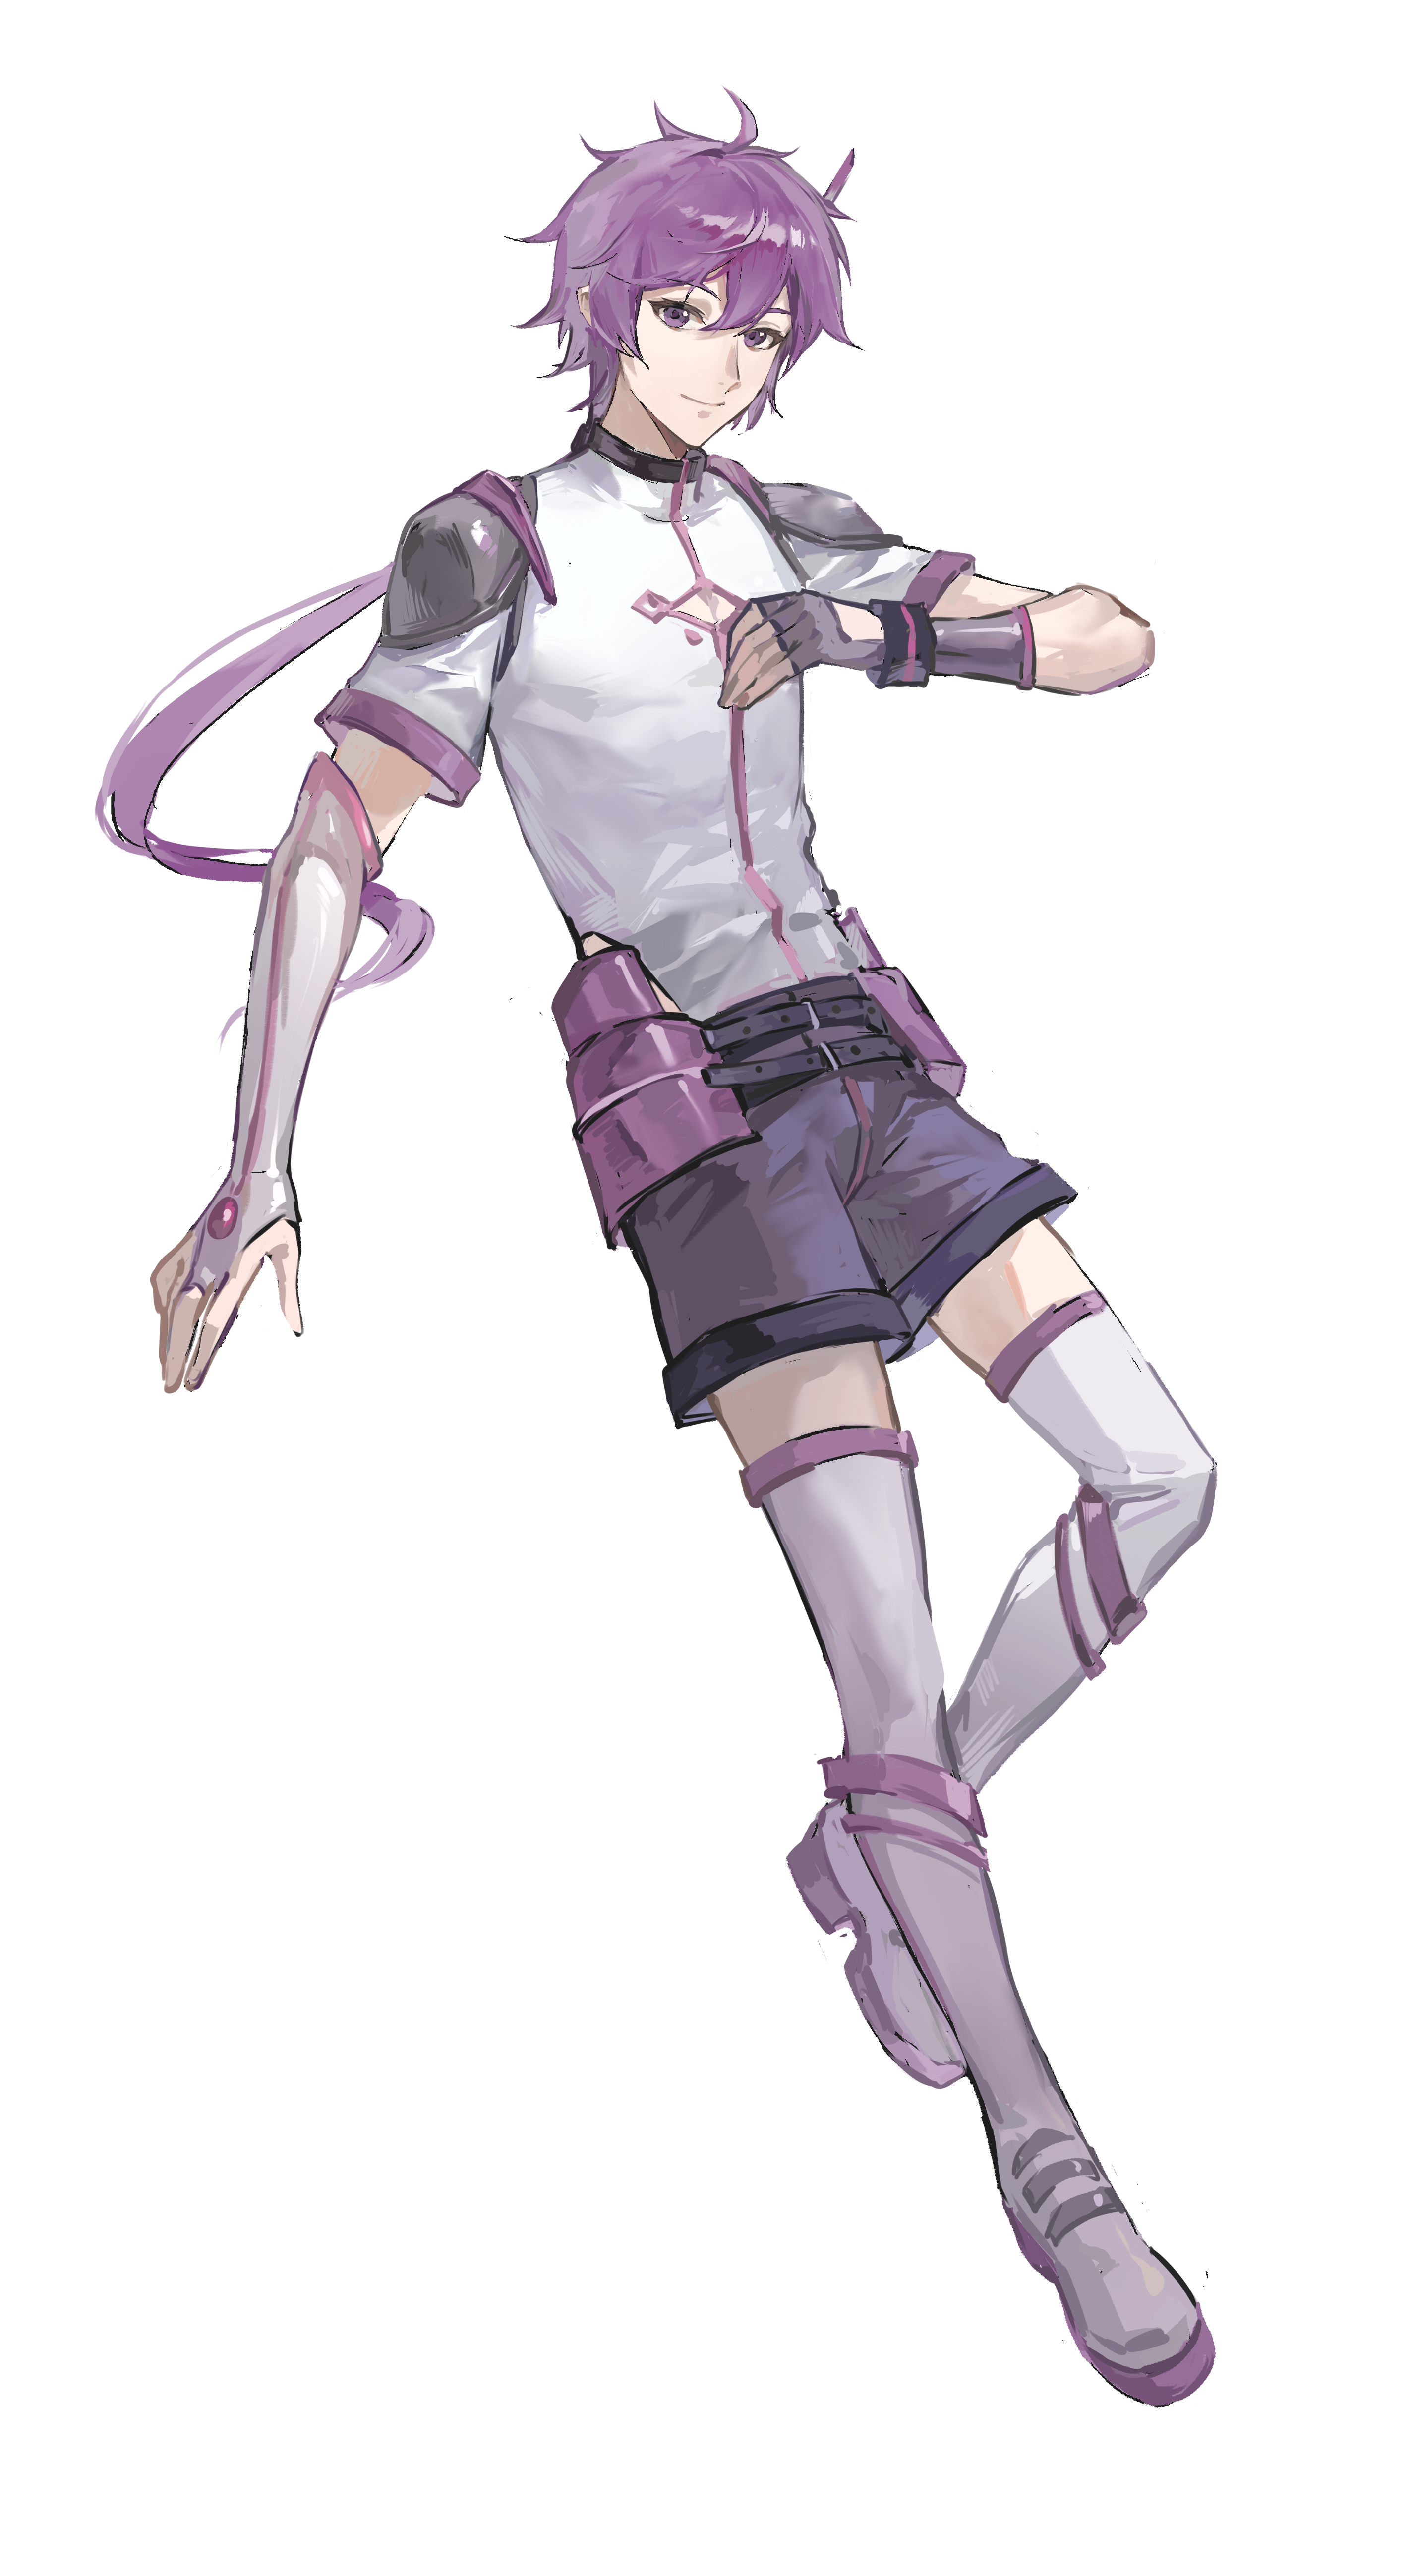
\includegraphics[height=1.82\linewidth,width=\linewidth]{zijingfull.png}}
    \end{minipage}%
    }
    
  
\end{flushleft}

  \adjustbox{valign=t}{
    \begin{minipage}[t]{0.35\textwidth}
      \vspace{-2em}
      \raisebox{-\height}[0pt][0pt]{
      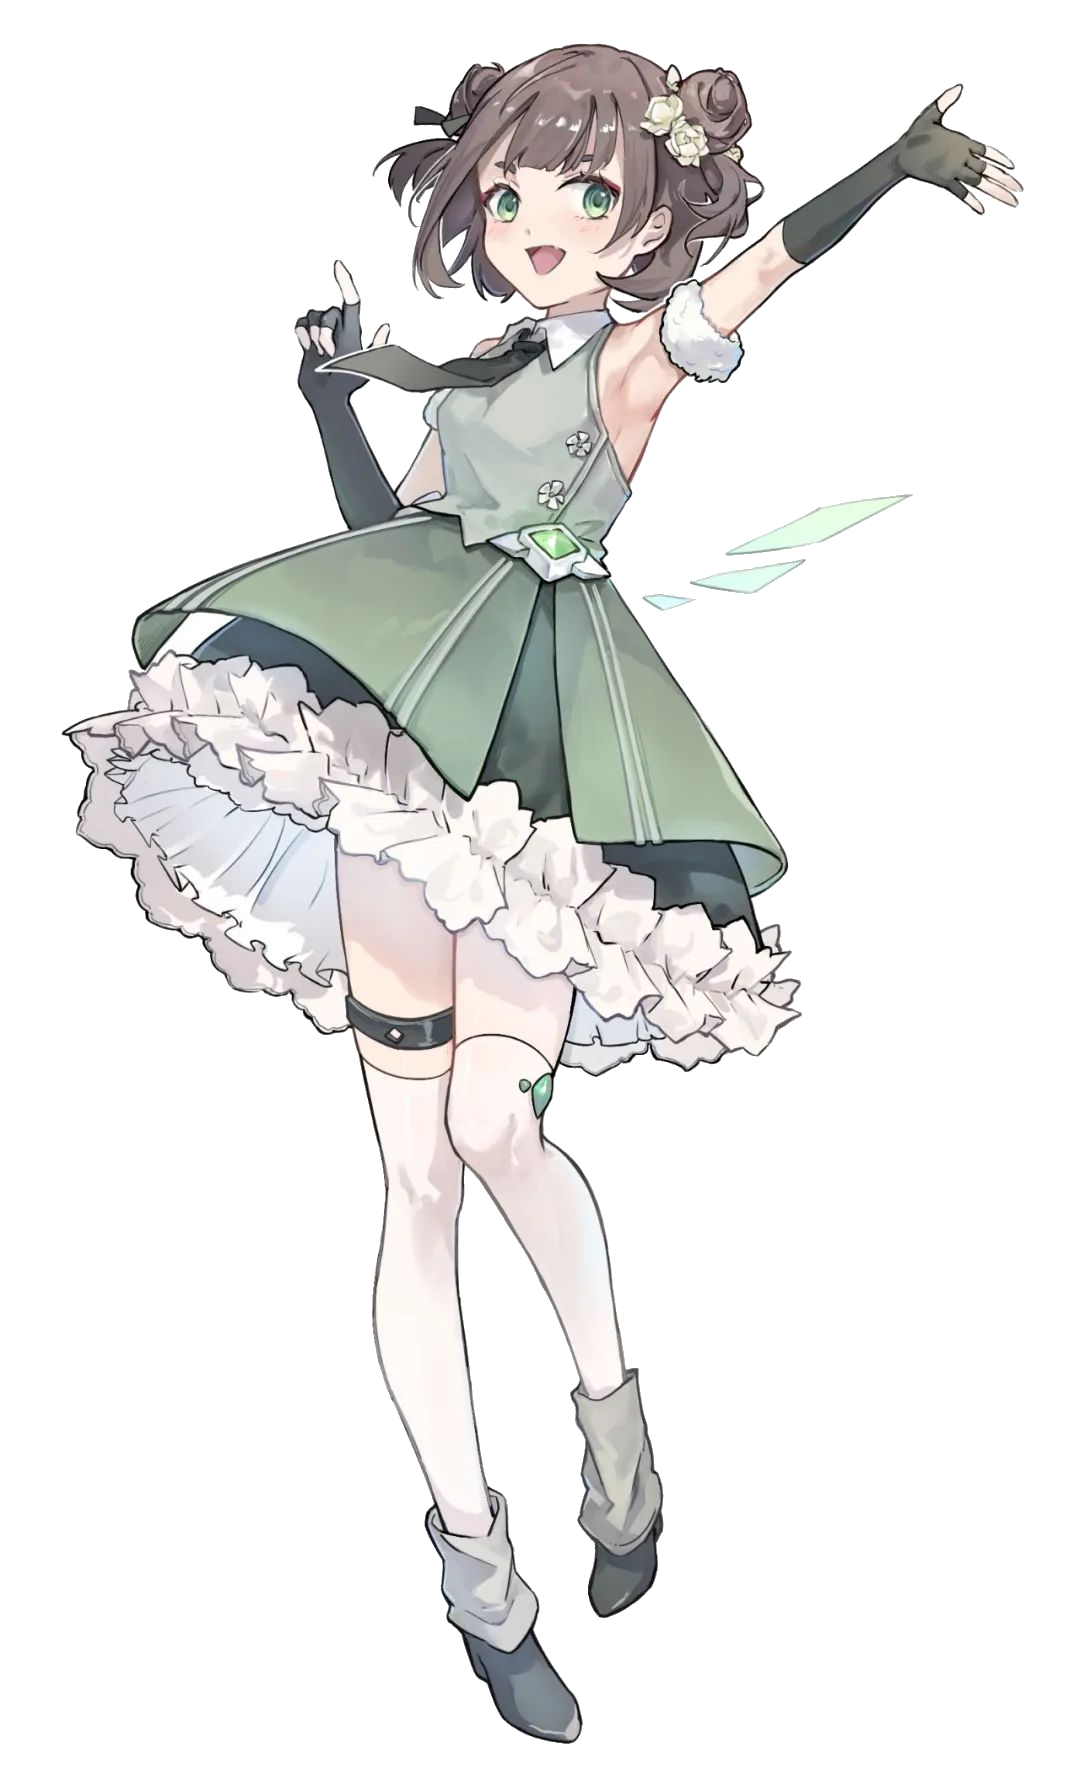
\includegraphics[width=0.85\linewidth]{qingfenfull.png}}
    \end{minipage}%
    }
    \hfill
    \adjustbox{valign=t}{
    \begin{minipage}[t]{0.55\textwidth}
        \section*{\Large\textbf{\textcolor{green!50!black}{清芬}}}
        \vspace{-1em}
        \subsection*{\normalsize\textbf{\textcolor{thuorange}{Meet Qingfen}}}
        \vspace{-0em}
        \small
      \chind 自幼便能歌善舞、希望带给大家开心和笑容的清芬加入次世代大家庭后,
      马上成为了社友们眼中最闪耀的偶像!\\ 
      \chind 作为次世代最小的看板娘,
      非常喜欢桃子和紫哥(虽然常常以玩笑掩饰自己的这份喜欢)。平时尤以捉弄桃子为乐,但是又会做非常多超好吃的甜点带给桃子,
      引得桃子对清芬死心塌地(?);\\ 
      \chind 日常中欢快跳脱的性格
      和舞台上闪闪发光的演出引得众人喜爱,
      但是也常常做出种种脱线的行为,让紫哥头疼不已……    
        \vspace{0.4em}
    \end{minipage}
    }
% 聊天对话部分
% 使用chatbubble命令创建对话气泡
% 语法:\chatbubble[位置]{头像}{昵称}{内容}{背景色}
\newpage 
\chatbubble[left]{taozi.png}{桃子没有在摸鱼}{%
大家好,这里是次世代的初代看板娘桃子\~{}
}{tao}
\chatbubble[left]{qingfen.png}{清芬}{%
大家好!我是次世代的看板娘清芬!
}{qing}
\chatbubble[right]{zijing.png}{紫荆}{
  我是紫荆。
}{zi}
\chatbubble[left]{taozi.png}{桃子没有在摸鱼}{%
那么什么是次世代呢?
}{tao}
\chatbubble[right]{zijing.png}{紫荆}{
那么什么是次世代呢?
}{zi}
\chatbubble[left]{qingfen.png}{清芬}{%
客服工号1911桃子为您解答:
}{qing}
\chatbubble[left]{taozi.png}{桃子没有在摸鱼}{%
?!
}{tao}
\chatbubble[left]{taozi.png}{桃子没有在摸鱼}{%
欸多\~{}咳嗯!次世代全称清华大学学生次世代动漫社,是,是……由两百多个兴趣部门组成的……
}{tao}
\chatbubble[left]{qingfen.png}{清芬}{%
……泛ACGN类兴趣社团(看稿子)
}{qing}
\chatbubble[right]{zijing.png}{紫荆}{
你俩……
}{zi}
\chatbubble[left]{taozi.png}{桃子没有在摸鱼}{%
咳嗯!次世代的一大特色就是丰富多彩的兴趣部门。从ACGN到运动养生,无论你对什么感兴趣,都可以在分部里找到你的同好!
}{tao}
\chatbubble[left]{qingfen.png}{清芬}{%
是的!即使没有找到组织,也可以秉着“三人成部”的原则,寻找同好,建立自己的兴趣部门!目前已经注册在案的有两百多个部门了\~{}
}{qing}
\chatbubble[right]{zijing.png}{紫荆}{
言归正传。接下来,让我们看一些社团资料,更加深入地了解次世代。
}{zi}
\newpage

\chatbubble[right]{zijing.png}{紫荆}{
以下是社团Q\&A示例。
}{zi}
\chatbubble[left]{guitarhero.png}{吉他英雄}{
  加入动漫社……是不是意味着要参加好多好多线下活动?要自我介绍?要上舞台?
  这个绝对做做做做做做做做不到!
}{default}

% 右侧聊天(用户B)
\chatbubble[right]{taozi.png}{12-桃子}{
 绝对没这回事\~{}我们所有的活动都是自愿参加的!当然,我们欢
 迎每一位社员的热情。但是就算只是来咖啡厅买一杯特调,来社庆做
 一枚静静的观众,或在群聊里默
 默收集好看的图片也都没问题!我们的宗旨就是玩得开心\~{}
}{tao}
  % 第一章:社团介绍
\input{chapters/2_activities.tex}  % 第二章:主要活动介绍
\chatbubble[left]{qiya.jpg}{奇犽}{
 次世代有哪些活动?
}{default}

\chatbubble[right]{taozi.png}{桃子}{
 次世代的活动真的超级多!常驻活动有每年一次的社庆晚会,每学期一次主题咖啡厅、
 乐队live、宅舞专场演出,以及各分部自发组织的活动,如绘画部的茶绘、动研部的新番研讨会、
 地下live部的应援例会、东方部的东方例会、Lolita部的茶话会、各个二游部的集体赌博
 (给赌博来个划掉的效果)抽卡等等;此外还会不定期掉落一些大牛的讲座分享
 (已经建设过丁丁框大大和匹诺曹大大了!)、圣诞例会、配音演员见面会等等。
 未来还会有更多的活动需要由你们来建设,快来和桃子一起搞波大的吧!
}{tao}

\chatbubble[left]{guitarhero.png}{吉他英雄}{
  加入动漫社……是不是意味着要参加好多好多线下活动?要自我介绍?要上舞台?
  这个绝对做做做做做做做做不到!
}{default}

% 右侧聊天(用户B)
\chatbubble[right]{qingfen.png}{清芬}{
 绝对没这回事\~{}我们所有的活动都是自愿参加的!当然,我们欢
 迎每一位社员的热情。但是就算只是来咖啡厅买一杯特调,来社庆做
 一枚静静的观众,或在群聊里默
 默收集好看的图片也都没问题!我们的宗旨就是玩得开心\~{}
}{qing}

\chatbubble[left]{zijing.png}{紫荆(四肢驯服中)}{
 不会跳舞可以加入宅舞部吗。?
}{zi}

\chatbubble[right]{taozi.png}{桃子}{
 当然可以!宅舞部很多都是0基础的朋友噢~只要热爱就可以加入,
 大家会一起学舞一起练习的(抱大腿)喜欢您来!
}{tao}

\chatbubble[left]{mortis.png}{若叶睦(Mortis 版)}{
 想加入创作部门,但无论乐队还是绘画、cosplay、宅舞,全~都不会!
}{default}

\chatbubble[right]{qingfen.png}{清芬}{
 没关系,大部分人都和你一样!正是因此,几乎每个创作部门招新时都会强调:
 我们部门从不拒绝零基础选手,我们有热心太太组成的资深团队,帮助每个虚心求教的萌新快速入门!
}{qing}

\newpage

\chatbubble[left]{konami.png}{(该用户未填写昵称)}{
 我的品味小众又独特,该如何在次世代找到同好呢?
}{default}

\chatbubble[right]{taozi.png}{桃子}{
 次世代最不缺的就是小众作品爱好者(此处应有一张部门全表),只要多水群,找不到同好比找到同好还难呢!
 此外,我们秉承“三人成部”传统,只要再有两位同好,就可以申请成立一个新部门\~{}如果你有感兴趣的领域
 还没有部门,欢迎来找我们哦!
}{tao}

\chatbubble[left]{shishangyou.png}{冻鳗领域大神}{
 如何向大家推荐我喜欢的作品?
}{default}

\chatbubble[right]{zijing.png}{紫荆}{
 有很多种方式。次世代动画研究会(简称动研部)会定期举办新番研讨会,这是安利作品、分享见解的最好机会。
 此外,次世代放映组每周都会组织放映会,现在加入放映部,完成登记和教室预约后,就可以申请放映自己喜欢的作品了。
}{zi}

\chatbubble[left]{wohenhaoqi.png}{好奇宝宝}{
 我也想为次世代的活动出一份力,我该如何成为帕鲁?
}{default}

\chatbubble[right]{qingfen.png}{清芬}{
 次世代组织部欢迎你的加入!组织部每周都会举办例会,分配下一周的工作任务。
 值得一提的是,所有任务都是自愿接受的,例会只来旁听也完全没问题\~{}
 在主题咖啡厅、社庆等大型活动前,组织部群里还会发布志愿者招募公告,填写问卷后就可以成为帕鲁啦!
 大型活动的帕鲁可能还会有神秘福利哦\~{}
}{qing}

\chatbubble[left]{rika.png}{极东魔术昼寝结社の夏社长}{
 次世代会和其他社团合作举办活动吗?
}{default}

\chatbubble[right]{zijing.png}{紫荆}{
 时常会有。次世代放映部每两周就会和学生科幻协会合作举办科幻电影放映会;主题咖啡厅也是外社
 联动的常客,荷月玩偶社、学生科幻协会等都曾是我们的联动对象。此外,学生电子音乐协会、学生推理协会
 也曾和我们有过合作。如果有任何想要进行外社联动的想法,欢迎联络组织部。
}{zi}

\newpage  % 第三章:社团Q&A
    \fontsize{23pt}{24pt}\selectfont
    \textbf{\textcolor{truepurple}{次世代cosplay舞台剧部}}\\
\vspace{0.7em}
  \adjustbox{valign=t}{
    \begin{minipage}[t]{0.25\textwidth}
      \vspace{-0.5em}
      \raisebox{-\height}{
      
\includegraphics[width=\linewidth]{部酱/cosplay舞台剧.png}}
      
      \picbox{\small ~~\ding{115} ~ cosplay舞台剧部酱~}
    \end{minipage}%
    }
    \hfill
    \adjustbox{valign=t}{
    \begin{minipage}[t]{0.65\textwidth}

        \normalsize
    \chind 大家好啊,这里是cosplay舞台剧部!\\
\chind 顾名思义,这里既有cosplay,又有舞台剧———是并集而不是交集。\\
\chind 部门的活动有许多,包括最盛大的社庆舞台剧节目、百团大战出cos、在动漫咖啡厅活动出cos、约漫展、约团片、约计划、约饭……\\
\chind 社庆的舞台剧节目上,我们有19年的命运石之门,21年的方舟走秀,24年的逆转裁判和25年的“苹果默示录”。\\
\chind 在百团大战中,社团会约好c楼的活动室方便大家化妆,一起在摊位上出cos也不社恐。在动漫主题咖啡厅中,我们还会设置符合主题的布景,让大家拍照使用。\\
\chind 大家可以组团去方舟ONLY、V家ONLY等漫展。\\

    
    \end{minipage}
    }
    \adjustbox{valign=t}{
    \begin{minipage}[t]{0.65\textwidth}

        \normalsize

\chind 约团片约计划什么的,只需要在群里说一声。万一成功了呢!这组JOJO黄金之风团片仅仅起源于一句话。并且结束以后一起去吃了披萨。\\
\chind 没出过cos,怎么办?尽管在群里提出问题吧!群内也有技术高超的妆娘、毛娘老师。试着在部门活动中迈出cosplay的第一步。\\
\chind 总之,欢迎所有对此有兴趣的同学加入!
\\  
    
    \end{minipage}
    }
    \hfill
  \adjustbox{valign=t}{
    \begin{minipage}[t]{0.25\textwidth}
      \vspace{-0.5em}
      \raisebox{-\height}{
      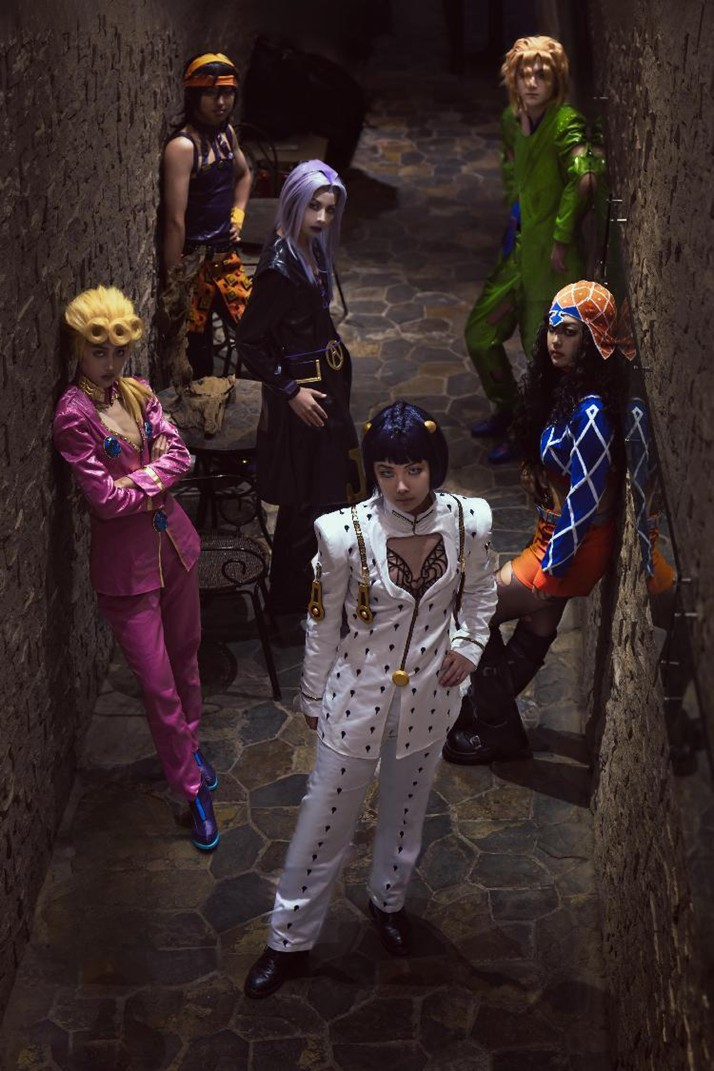
\includegraphics[width=\linewidth]{cos部3.jpg}}
      
      \picbox{\small ~~\ding{115} ~ JOJO黄金之风团片~}
    \end{minipage}%
    }
      \adjustbox{valign=t}{
    \begin{minipage}[t]{0.45\textwidth}
      \vspace{-2.5em}
      \raisebox{-\height}{
      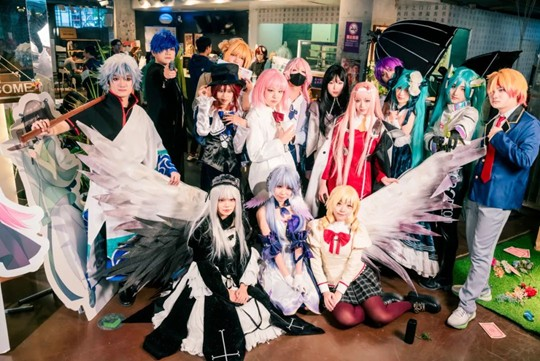
\includegraphics[width=\linewidth]{cos部1.jpg}}
      
      \picbox{\small \ding{115} ~ 2024咖啡厅coser合影~}
    \end{minipage}%
    }  \adjustbox{valign=t}{
    \begin{minipage}[t]{0.45\textwidth}
      \vspace{0.5em}
      \raisebox{-\height}{
      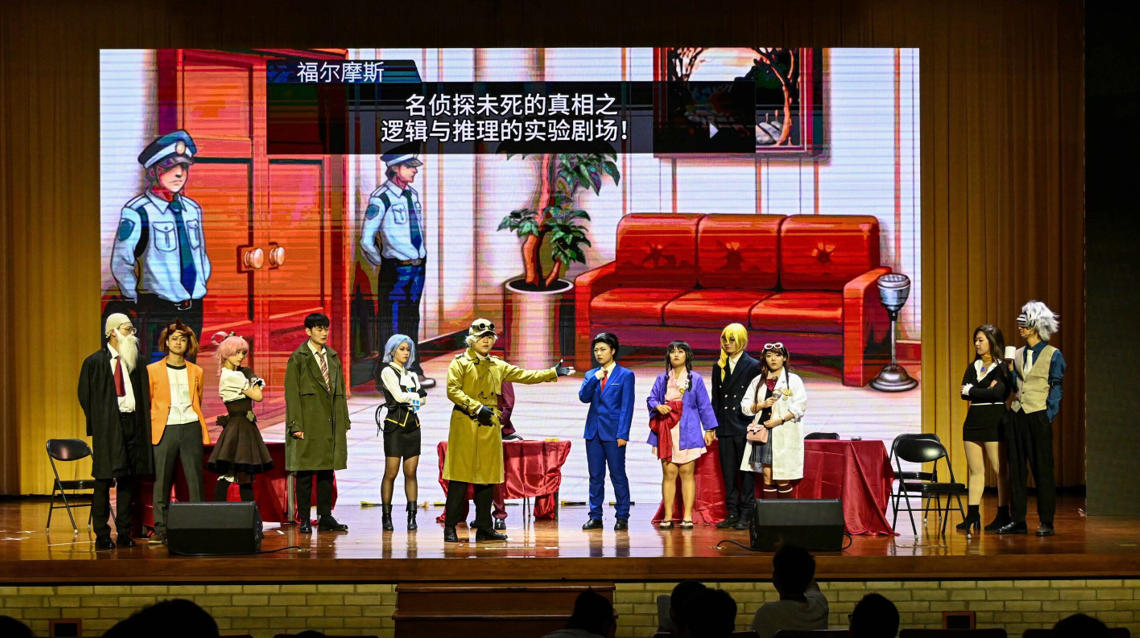
\includegraphics[width=1.1\linewidth]{cos部2.jpg}}
      
      \picbox{\small ~~\ding{115} ~ 2024社庆舞台剧《逆转裁判》~}
    \end{minipage}%
    }
    \newpage
    \fontsize{23pt}{24pt}\selectfont
    \textbf{\textcolor{truepurple}{次世代周边交易部(谷子部)}}\\
  \adjustbox{valign=t}{
    \begin{minipage}[t]{0.25\textwidth}
      
      \raisebox{-\height}{
      
\includegraphics[width=\linewidth]{谷子部1.png}}

    \end{minipage}%
    }
    \hfill
    \adjustbox{valign=t}{
    \begin{minipage}[t]{0.7\textwidth}


        \normalsize
\vspace{0.5em}
\chind “终于上大学了,入坑这么多年,终于能支配财力买点喜欢的周边啦,让我看看——”“诶这个好贵,诶那个怎么像假的,诶这个预定是怎么回事啊”“问题好多不敢下手了o(╥﹏╥)o\ldots”\\
\chind 别急别怕!这里是次世代周边交易部,资深玩家专业团队在线答疑解惑,无论是吧唧爱好者,还是手办收藏家,无论是想打探情报,还是想挥手爆米,都能在这里找到所需所寻☆( ̄▽ ̄)/\$


    
    \end{minipage}
    }
    \normalsize
    \par
    \vspace{0.5em}
\chind 次世代周边交易部,成立于2025.03.10,别名谷子部,顾名思义,我们是一个和\textbf{ACG周边制品}相关、和¥相关的分部,在活跃中展现了极具特色的功能性。
    \adjustbox{valign=t}{
    \begin{minipage}[t]{0.6\textwidth}


        \normalsize

\chind 本部成立的初心,也是本部第一部活,即构建一个和谐实在的\textbf{小二手市场}。
在这里,大家可以按需挂出或收入周边,包括徽章吧唧、立牌、色纸、书籍、
钥匙扣、手办、挂画等现货或预售转单。这里都是自己人,\textbf{可信度高};当面交易,
\textbf{优惠免邮,即时便捷};交流友善,和谐舒心。作为本模块的延伸,
谷子部还会在\textbf{百团展出}各种周边,并在\textbf{咖啡厅同步设置摊位}。

    
    \end{minipage}
    }  
    \hfill
\adjustbox{valign=t}{
    \begin{minipage}[t]{0.35\textwidth}
      
      \raisebox{-\height}{
      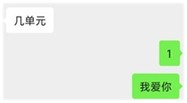
\includegraphics[width=\linewidth]{谷子部2.jpg}}

    \end{minipage}%
    }
    \par
\vspace{0.5em}
\chind 随着部门参与人数增多,依大家所需,谷子部更新出第二部活——\textbf{情报模块}。以资深玩家为中心,谷子部可以为大家提供丰富的\textbf{信息渠道以及购买渠道},为大家\textbf{比价选价,辨别真伪},省钱省心。如各类手办如何购买,如何闲鱼收中古手办,IP限时联动信息,以及BW漫展抢票等等。\\
\chind 在情报模块中,\textbf{线下探店(“开图”)}得到极大的兴趣投入,也自然成为了谷子部第三部活。这一部活中,社友或独行或结伴,去探索城市内各种\textbf{手办店、漫画轻小说店、IP谷子店},足迹遍布京、津、沪、成都、广州、哈尔滨等,最下方为京汇总图及实拍例(上海龙之梦-桐叶pop up,悦荟-深睡羊-异世界情绪展柜)。\\
\chind 周边交易、情报分享、线下开图……谷部活动绝赞上新中,希望大家来一同建设。欢迎各位新老社友加入谷子部,获取更多即时情报\~{}
\par
\adjustbox{valign=t}{
    \begin{minipage}[t]{0.6\textwidth}
      \vspace{0.6em}
      \raisebox{-\height}[0pt][0pt]{
      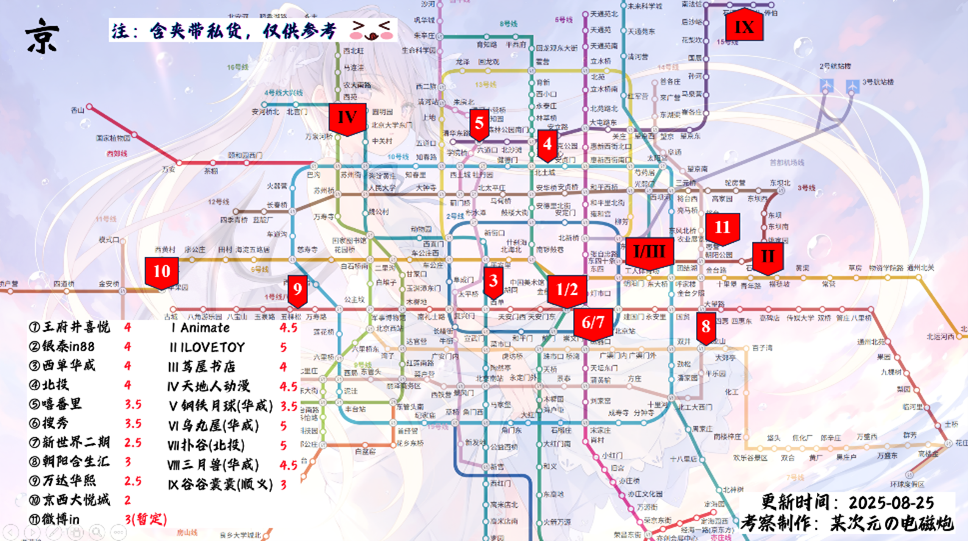
\includegraphics[width=\linewidth]{谷子部3.png}}
    \end{minipage}%
    }
    \hfill
      \adjustbox{valign=t}{
    \begin{minipage}[t]{0.35\textwidth}
      \vspace{-0.5em}
      \raisebox{-\height}{
      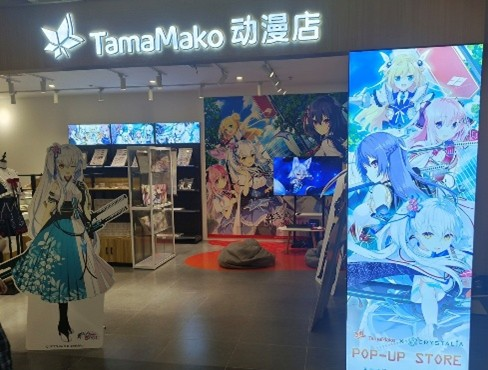
\includegraphics[width=\linewidth]{谷子部4.jpg}}
      \vspace{1em}
      \raisebox{-\height}[0pt][0pt]{
      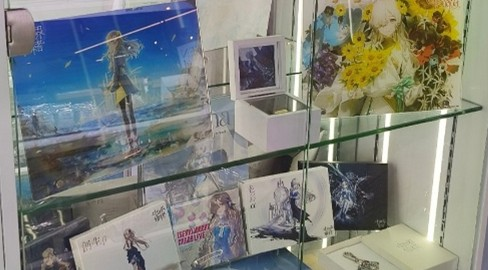
\includegraphics[width=\linewidth]{谷子部5.jpg}}
    \end{minipage}%
    }
\newpage
    \fontsize{23pt}{24pt}\selectfont
    \textbf{\textcolor{truepurple}{次世代心憩部}}\\
    \vspace{0.7em}
  \adjustbox{valign=t}{
    \begin{minipage}[t]{0.2\textwidth}
      \vspace{-0.2em}
      \raisebox{-\height}[0pt][0pt]{
      
\includegraphics[width=1.1\linewidth]{心憩部.jpg}}
    \end{minipage}%
    }
    \hfill
    \adjustbox{valign=t}{
    \begin{minipage}[t]{0.7\textwidth}

        \small
\chind 欢迎加入心憩部/心理支援部捏!\\
\chind 本部建立的初衷是:互帮互助,让自己的生活更好一些——我们讨论如何改善身心问题与精神困扰,
也欢迎遇到困境的同学群友一起分享从看诊用药心得,到心理调节资源的各种知识,以及日常生活的体验与感想~\\
\chind 为什么会想在次世代动漫社里,建立一个以心理健康为主题的,听上去像抱团取暖(但其实并不是x)的社群呢?\\
\chind 加入次世代一段时间后,我始终忘不了一些社友在一些分部里面,倾诉自己遇到的学习生活困境
,回应他们的却或是无视或是委婉劝止(这里不是讨论沉重话题的地方),或是更多负面悲观的螺旋中。
这样做并不能让现实生活中的问题消失,并且就算有人提出了有价值的信息,也会旋即被水群的日常活动淹没乃至遗忘。\\

    
    \end{minipage}
    }
    \small

    \chind 我希望能真正帮助到大家,我也不认为逃避或者愤世嫉俗才是二次元的主基调,
成长和互帮互助一样是,因此有了这个试图分享心理健康资源,以及提供人文关怀和相互启发的心憩部,
或者也可以叫心理支援部(只是后者可能看起来像是走投无路的同学才会加入的样子,所以改成了前者)\\
\chind \textbf{爱是永不止息,无论在什么地方,以什么方式。}
\\  
    \newpage
    \fontsize{23pt}{24pt}\selectfont
    \textbf{\textcolor{truepurple}{次世代米游杂食铺}}\\
    \vspace{0.7em}
  \adjustbox{valign=t}{
    \begin{minipage}[t]{0.25\textwidth}
      \vspace{-0.2em}
      \raisebox{-\height}[0pt][0pt]{
      
\includegraphics[width=\linewidth]{米游铺1.jpg}}
    \end{minipage}%
    }
    \adjustbox{valign=t}{
    \begin{minipage}[t]{0.65\textwidth}

        \small
\chind 喵喵喵\verb|~~~(^▽^)ゞ| 各位舰长旅行者律师开拓者寻梦者绳匠大家好呀,这里是米家杂食铺!\\
\chind 本部定位为米游社区分层中偏向享受游戏本身而远离焦虑和纷争的部分,所以将对引战/内鬼/拉踩行为做出更加严苛的限制,让我们一起营造出一个mmr友好的小圈吧\~{}\\
\chind 目前群里已有大佬们制作了赛飞儿等AI聊天bot可供大家免费使用,让我们来赛博撸猫吧\~{}\\


    
    \end{minipage}
    }
    \small

\adjustbox{valign=t}{
    \begin{minipage}[t]{0.7\textwidth}

        \small
\chind 此外,本部设立两红包奖项,一为安慰奖,一般在每月所有卡池更新后为群最非颁发约等于一张小月卡的小红包,不要因为抽卡而坏了游戏的性质喔;二为群活跃增值奖,一般在积极参与相关活动并带动群内积极讨论活跃时候颁发。\\  
\chind 欢迎大家来建设部活、分享二创和cos以及各种群帮帮等,让这个小部门热闹起来吧。\\
\chind 所以赶快来加入我们吧\~{}
    \end{minipage}
    }
  \adjustbox{valign=t}{
    \begin{minipage}[t]{0.2\textwidth}
      \vspace{-0.2em}
      \raisebox{-\height}[0pt][0pt]{
      
\includegraphics[width=1.1\linewidth]{米游铺2.jpg}}
    \end{minipage}%
    }
    \hfill

\vspace{2em}    
\fontsize{23pt}{24pt}\selectfont
\textbf{\textcolor{truepurple}{次世代星露谷物语部}}\\
\vspace{0.2em}
\small
\chind 你说得对,但是星露谷物语是一个牧场类的RPG游戏,你继承了爷爷在星露谷的农场,
但是你手头上只有最基础的农具和少许金钱,你得靠此开始你的新生活。
你能把这片杂草丛生的田地变成繁荣的家园吗?\\
\chind 欢迎各位老乡加入,也欢迎感兴趣准备入手的新玩家捏\~{}
  % 第四章:分部介绍
\newpage
\normalsize

\chatbubble[right]{Koyou.png}{22-Koyou 深度砖工}{
没有加入你社的话我大学生活估计会少大半乐趣。
}{zi}

\chatbubble[left]{阿茗.png}{22-阿茗不吃鱼~~25届副社长、宅舞部部长+组织部重度依赖\emoji{💜}}{%
跳舞很开心!搞cos很开心!拍照很开心!\\办活动很开心!大自习很开心!一起玩很开心!\\
欢迎加入宅舞部一起跳舞(幻想n年后宅舞部什么样子)\\
顺便祝大家早日脱单(抓走组织部长x)
}{default}

\chatbubble[right]{展颜.png}{22-展颜 \emoji{🐳}}{
\emoji{💜👍💃👍👏👏🙌👏👏🎉🎉🎉💃💃💃👍👍👍}
}{zi}

\chatbubble[left]{江枫.png}{14-江枫~~18届社长}{%
我的本科四年也是在次世代的四年,感觉每天做的事见的人度过的时光都和次世代紧紧相连着。
可以说次世代在某种程度上塑造了我,也深深地影响着离开校园的我。\\
希望次世代的家人们都能在这里获得属于自己丰满的美好的回忆~
}{default}

\chatbubble[right]{雨绫.png}{21-雨绫~~虽然喜欢的很多但既然是东方部管理所以大家来搞东方(?}{
次世代仿佛一个坚实的锚点,在每个人不一定一帆风顺的大学生活中,或许平时很难意识到,
事后回想才会发现原来平日的悲欢里都有它的影子。要相信在这个形形色色的人交织而成的团体中,
一定可以寻找到值得你珍视的线哦。
对了,在校期间一定要参与一次社庆吧,把你的热爱告诉所有人,留下独属于自己的痕迹!
}{zi}

\chatbubble[left]{寒月.png}{19-寒月}{%
开学的时候从百团大战加入的次世代,这里个个都是人才,说话又好听!找到了很多游戏、动漫同好,水群花了很多时间!
}{default}

\chatbubble[right]{沙包.png}{10-沙包}{
好怀念紫荆的麻辣香锅。
}{zi}

\chatbubble[left]{天海兰.png}{17-天海兰~~无限想念华子的毕业社畜学长}{%
感谢次世代,尤其是次世代东方部的伙伴们,曾经一起开例会,与全市车万人相聚,一起出发听幻奏盛宴,去玩东方only,这些记忆闪耀了我的大学时光。
}{default}

\chatbubble[left]{梧桐明夜.png}{20-梧桐明夜~~绘画部退休部长}{%
\chind 次世代是一个实现梦想的故事。从最早到这里了寻找一起搞彩虹小马的人,到在绘画部学画画,
再到进组织部干活、上台讲相声,我在次世代的每一步都走得出乎意料却充满获得感。
最早的时候,在次世代参加的每一次活动都会有新的悸动。总会产生我想在次世代完成这个,参与那个的期待。
顺着这些期待走去,在快乐的时光中,它们也一个个变成了现实。画了海报、上了社庆、当了部长,
总能看到一个个悸动开花结果。

\chind 曾记得一位社友说过:“次世代不是给人分发任务的地方,而是发现有谁想要做什么,
然后利用社团资源帮他实现想法的地方。”在次世代,只要敢想就能敢做。
在这里你能看到关于动漫和大学社团的所有幻想变成三次元的真实。

\chind 次世代也是一个找到自己价值的地方。丰富多彩的活动背后是每位社友的鼎力支持和倾情付出。只要你愿意成为其中的一部分,
总会有适合你的岗位,让你在社团活动中留下独属于自己的烙印。每次办完大型活动,
我都有一种身处热血番末尾的感觉。看着身为Staff的大家在散场音乐中合影,互道一声辛苦,
收拾自己的东西奔向聚餐。

\chind 你的每个闪光点都是次世代急需的宝藏,哪怕你自己都不曾意识到。
部门拟人的部酱企划本来是我一时兴起自娱自乐的产物,用于表达我入社四年来在各个部门的所见所感。
没想到能得到社友们的厚爱,甚至变成了DV剧搬上社庆。只要献出你独特的爱,在次世代,总会有用你的钥匙才能打开的门锁。

\chind 次世代绘画部是一个家一样的地方。大家在里面各自发画,相互夸夸,一问一答,相约线下。
最近的每次茶绘都能挤满C楼的教室。大家说说笑笑,交换无料,在同一张画布上描绘自己的心迹。绘画部的人都很温柔,
绘画部的空气都很清新。无论你是大触还是新手,都能在这里找到归属。
}{default}

\chatbubble[right]{撒旦.png}{18-撒旦~~被迫隐身虾饺传说}{
Helden sterben nicht!祝次世代的大家永远不死\~{}
}{zi}

\chatbubble[left]{TerryWScheler.png}{23-TerryWScheler~~加入原神部谢谢喵}{%
希望能像玛拉妮一样每天都很乐观
}{default}

\chatbubble[right]{砂53.png}{25-砂$5^3$~~究极百合骑士}{
出勤时受到博士老登感化加入次世代\\
应该是你社为数不多百团前就加入的小登\\
(是的 主播开学第四天就穿着系服出勤了喵)\\
诸君,请玩音游吧!
}{zi}

\chatbubble[left]{四号线.png}{21-四号线~~关注星瞳official谢谢}{%
路过的观众,请容我向您介绍一位出色的虚拟偶像-星瞳,关注星瞳喵,关注星瞳谢谢喵。星瞳是 FPS 游戏高手、全民 k 歌黄金段位拥有者、舞者、歌手、小说家、相声演员、画师。
}{default}

\chatbubble[right]{无解.png}{20-无解~~加入东方部/轻小说部/日语学习部谢谢喵}{
在你社留下了很多回忆,也认识了很多朋友,是和大家一起玩的回忆支撑我走过了在校的时光。
次世代这种纯粹地在“玩”而没有什么内卷和功利心的地方是非常珍贵的,
欢迎大家在这里走错(啊不)迈出自己的大学第一步
}{zi}

\chatbubble[left]{疾风.png}{20-疾风}{%
其实一开始没打算加学校动漫社这种现充俱乐部(刻板印象)的,
不过被社友朋友介绍的三人成部吸引于是还是速速入社摇人成立了IDOLiSH7部哈哈哈。
因为自由宽松的建部和入部制度,次世代有着多种多样的兴趣部门且可以同时参加,
得益于此,即便是我这样的社恐老废宅,只需要一点勇气,也能在次世代体验了第一次参本、
参与社庆舞台灯光工作、组织JSD48×IDOLiSH7舞蹈节目、参演舞台剧(虽然因为疫情变DV剧了)和配音节目、
和社友出去唱K……感谢次世代,给予了我很宝贵的回忆。
}{default}

\chatbubble[right]{恒斌.png}{18-恒斌~~(曾)ktn单推人}{
加入次世代,走错人生第一步(bushi\\
然后加入galgame部,走错人生第二步(bushi\\
我很庆幸我加入了次世代,加入了galgame部,在这里我收获了非常快乐的时光,也结识了很多朋友,十年后的我,会更加感谢当初的决定吧\\
欢迎新来的朋友们,galgame部这边请
}{zi}

\chatbubble[left]{晓雾.png}{18-晓雾~~我要看一辈子动画片}{%
\chind 本科的时候因为太沉迷学习(没有时间)和愧于自己二次元浓度不足(沉淀不够)而一直没想过动漫社的事情,
直到一年半前的百团突然心血来潮走错了大学的第不知道多少步!
遇到了很多有意思的社友,也参加了一些有意思的活动。在动研部邂逅一众冻鳗高手;
在放映部从社恐观众进化为可以塞私货的放映员;在京阿尼部和粳米们一起听音乐会、一起K歌,
并以此为契机下定决心开始学霓虹语和学歌,也在放映会狠狠加入京阿尼的动画片!\\
\chind 最死而无憾的是尽心尽力办了最最豪华的京紫剧场版放映会,
最残念的是精心准备的京紫放映推送因为不可抗力没能留在你社公众号上QAQ。
立个flag,明年春天一定要放四谎口牙,我永远喜欢薇尔莉特和宫园薰(不要问为什么包括头像都是金毛我也不知道)!
总之下辈子也要加入次世代,这辈子就先组一辈子动漫社吧!
}{default}

\chatbubble[right]{shiro.png}{22-shiro~~福圆美里痴一枚}{
\chind 大家好,我是shiro,我已经是一个入社三年的老东西了。刚入社的时候我还是一个什么都不懂的小毛孩,现在已经变成了…好像也没什么变化(。这几年我真的收获了很多快乐,结交了很多朋友。在社友的安利下我成功地入坑galgame,并成功地变成了福圆美里吃,总感觉我这辈子有了(?\\
\chind 让我印象最深刻的,是我参加的第一次新番研讨会。当时的讨论很热烈,大家也都很热情(现在的线下新番研讨会更热情了),我第一次由衷地感觉到,原来我的同类也不少。\\
\chind 也希望你也能在次世代动漫社收获一份快乐。
}{zi}

\chatbubble[left]{谭秀.png}{25-谭秀}{%
我是五字班的新生,虽然看的番不多,也不玩二游,但一直对二次元很感兴趣。
我特别喜欢东方project,无论是stg新作,还是优秀的同人创作,都会努力去品味,
体会大家的创作热情。希望在来到大学后,能结识很多同好,徜徉于二次元的海洋!
}{default}

\chatbubble[right]{崇山珞石.png}{20-崇山珞石~~2023-2024社长}{
非常感谢次世代这个温暖的大家庭给了我一个快乐的港湾,希望大家可以珍惜、享受、建设这个大家庭。
}{zi}
\chatbubble[left]{异步.png}{23-异步~~加入水木wota艺部来打光棒包教包会}{%
作为追随某神秘学长入社的小登,感激次世代良好的氛围给予了众多小众爱好发展的土壤。回想起我刚刚入社时四处打听有没有学长会打wota艺能不能教教我的往事,会觉得自己成为了曾经向往的那个存在。希望复活的wota艺部能给每一个憧憬舞台渴望闪耀的新人提供一个不错的方向。
}{default}

\chatbubble[right]{千枫.png}{24-千枫~~加入音游部wota艺部星铁部谢谢喵}{
这一年来蹭活动蹭的很开心,在组织部搬砖也搬的很开心!感谢次世代收留了这般内向而社恐的我,让我在大学重拾了高中同窗般的温暖!期待与次世代的第二年
}{zi}

\chatbubble[left]{Line.png}{24-Line}{%
或许以后我们会散落不同的城市,会在通勤地铁上疲倦地刷着新番,但永远会记得——曾有群中二病战友,陪我们把幻想浇铸成真。希望大家都能在次世代找到一种归属感,玩得开心。
}{default}

\chatbubble[right]{zijing.png}{紫荆}{
以下是社员寄语示例。
}{zi}
\chatbubble[left]{qingfen.png}{22-清芬}{%
紫哥桃子姐带我入社已经三年啦! 次世代的社友个个都是人才,说
话也好听,玩得很开心呢。要说印象最深刻的当然是第一次 idolive
宅舞专场我的舞台初体验啦,但是当然不仅限于此,每一天都很
欢乐呢! 最喜欢次世代的大家了!
}{qing}  % 第五章:社员寄语
\newpage

\end{document}